\documentclass[aspectratio=169,11pt,hyperref={colorlinks=true}]{beamer}
% https://github.com/zr-tex8r/BXcjkjatype/blob/master/README-ja.md
\usepackage[whole]{bxcjkjatype}
\usetheme{boxes}
\setbeamertemplate{navigation symbols}{}
\definecolor{suse}{RGB}{2, 211, 95}
\definecolor{susedark}{RGB}{13, 44, 64}
\definecolor{linkcolor}{RGB}{13, 44, 255}
\setbeamercolor{titlelike}{fg=suse}
\setbeamercolor{structure}{fg=suse}
\hypersetup{colorlinks,urlcolor=suse}
\setbeamertemplate{footline}[frame number]
% Inserting graphics
\usepackage{graphicx}
% Side-by-side figures, etc
\usepackage{subfigure}
% Code snippits
\usepackage{listings}
% Color stuff
\usepackage{color}
% underline
\usepackage{soul}
% calc
\usepackage{calc}

\usepackage{amsmath}
\usepackage{tikz}
\newcommand\RBox[1]{%
  \tikz\node[draw,rounded corners,align=center,] {#1};%
}
\usepackage{hyperref}
%\usecolortheme{buzz}
%\usecolortheme{wolverine}
%\usetheme{Boadilla}
\usepackage[T1]{fontenc}
%\usepackage{fontspec}
%\usepackage[expert, deluxe]{otf}

\definecolor{mygreen}{rgb}{0,0.6,0}
\definecolor{mygray}{rgb}{0.5,0.5,0.5}
\definecolor{mymauve}{rgb}{0.58,0,0.82}


%\usepackage{CJK}
%\pdfmapline{=genshingothic@Unicode@ <genshingothic.ttf}
% bxcjkjatype
%\setgothicfont[<ID>]{<フォントファイル名>}
%\setgothicfont{/Users/foo/Library/Fonts/genshingothic.ttf}
%\setgothicfont{/Users/foo/Library/Fonts/NotoSansCJKjp-Regular.otf}
%\setgothicfont{/Users/foo/Downloads/genshingothic-20150607/GenShinGothic-P-Normal.ttf}
%\setgothicfont{/Users/foo/Downloads/genshingothic-20150607/GenShinGothic-Regular.ttf}
%\setgothicfont{hiragino.ttc}
\setgothicfont{mplus-1p-regular.ttf}
\setCJKfamilydefault{\gtdefault}
%\setCJKfamilydefault{\mcdefault}
%\CJKforce{abcdefghijklmnopqrstuvwxyzABCDEFGHIJKLMNOPQRSTUVWXYZ}


\lstset{%
  backgroundcolor=\color{susedark},   % choose the background color; you must add \usepackage{color} or \usepackage{xcolor}
  breakatwhitespace=false,         % sets if automatic breaks should only happen at whitespace
  breaklines=true,                 % sets automatic line breaking
  captionpos=b,                    % sets the caption-position to bottom
  commentstyle=\color{suse},  % comment style
  extendedchars=true,              % lets you use non-ASCII characters; for 8-bits encodings only, does not work with UTF-8
  keepspaces=true,                 % keeps spaces in text, useful for keeping indentation of code (possibly needs columns=flexible)
  keywordstyle=\color{blue},       % keyword style
%  otherkeywords={*,...},           % if you want to add more keywords to the set
  numbersep=5pt,                   % how far the line-numbers are from the code
  numberstyle=\tiny\color{mygray}, % the style that is used for the line-numbers
  rulecolor=\color{white},         % if not set, the frame-color may be changed on line-breaks within not-black text (e.g. comments (green here))
  showspaces=false,                % show spaces everywhere adding particular underscores; it overrides 'showstringspaces'
  showstringspaces=false,          % underline spaces within strings only
  showtabs=false,                  % show tabs within strings adding particular underscores
  stringstyle=\color{suse},   % string literal style
}

\setbeamerfont{caption}{series=\normalfont,size=\fontsize{6}{8}}
%\setbeamerfont{caption}{series=\normalfont,size=\large}
\setbeamertemplate{caption}{\raggedright\insertcaption\par}

\setlength{\abovecaptionskip}{0pt}
\setlength{\floatsep}{0pt}

%%%%%%%%%%%%%%%%%%%%%%%%%%%%%%%%%%%%%%%%%%%%%%%%%%%%%%%%%%%%%%%%%%%%%

\author[Masayuki Igawa]{%
    \texorpdfstring{%
            \centering
            Masayuki Igawa\\
            \href{mailto:masayuki@igawa.io}{masayuki@igawa.io}\\
            \texttt{masayukig on
              \href{https://freenode.net/}{Freenode},
              \href{https://github.com/masayukig}{GitHub},
              \href{https://twitter.com/masayukig}{Twitter},
              \href{https://www.linkedin.com/in/masayukig/}{LinkedIn}}
    }
    {Masayuki Igawa}
}
\date{\href{https://containerdays.jp/timetable.html}{December 04, 2018}}
\def\place#1{\def\@place{#1}}
\place{\href{https://containerdays.jp/timetable.html}{@JapanContainerDays v18.12}}

%\vspace*{10pt}
\title[k8s-the-hard-way
  \hspace{4em}\insertframenumber/\inserttotalframenumber]{\Huge{Kubernetes The Hard Way}}

\setbeamercolor{background canvas}{bg=susedark}
\setbeamercolor{titlelike}{fg=white}
\setbeamercolor{structure}{fg=white}
\setbeamercolor{normal text}{fg=white}

\begin{document}
%\setbeamertemplate{background canvas}{
\includegraphics[width=\paperwidth,height=\paperheight]{images/opensuse_base.png}}
{%
% \setbeamertemplate{background canvas}{
\includegraphics[width=\paperwidth,height=\paperheight]{images/opensuse_preface.png}}
\setbeamertemplate{footline}{}
\setbeamercolor{background canvas}{bg=susedark}
\begin{frame}[noframenumbering]
  \hypersetup{colorlinks,urlcolor=suse}
  \setbeamercolor{author}{fg=white}
  \setbeamercolor{date}{fg=white}
  \setbeamercolor{place}{fg=white}
  \titlepage{}
  \centering
  \@place \par
  \href{https://bit.ly/k8s-the-hard-way-jkd-v1812}{https://bit.ly/k8s-the-hard-way-jkd-v1812}
  \begin{flushright}
    \tiny\href{https://creativecommons.org/licenses/by/4.0/}{This work
      is licensed under a Creative Commons Attribution 4.0
      International License.}~
\includegraphics[scale=0.3]{images/cc_by.png}
  \end{flushright}
\end{frame}
}

\section{Agenda}
\begin{frame}
  \frametitle{Agenda}
  \begin{enumerate}
    \item 自己紹介
    \item 今日のゴール
    \item \bf{Kubernetes The Hard Way} とは?
    \item 結論
    \item 今後の展望
    \item まとめ
  \end{enumerate}
\end{frame}

\section{DISCLAIMER}
\begin{frame}
  \frametitle{DISCLAIMER}
  \Huge{\bf{この内容は個人の見解であり、所属する組織・団体を代表するものではありません。}}
\end{frame}

\section{Who I am?}
\begin{frame}
  \frametitle{Who I am?}
  \begin{itemize}
    \item 所属企業:2017.3- SUSE/Novell Japan
    \item 仕事/肩書: Senior Software Engineer/Open Source Programmer
      \begin{itemize}
        \begin{scriptsize}
        \item \href{https://www.openstack.org/}{OpenStack}
          \href{https://wiki.openstack.org/wiki/QA}{QA} Up/Downstream development, Core Reviewer
        \item[]
          (\href{https://docs.openstack.org/developer/tempest/}{Tempest},
          \href{http://status.openstack.org/openstack-health/}{OpenStack-Health},
          \href{https://docs.openstack.org/developer/subunit2sql/}{Subunit2SQL},
          \href{https://docs.openstack.org/developer/stackviz/}{Stackviz}),
          \href{http://stackalytics.com/?user_id=igawa&release=all&metric=all}{stackalytics.com/?user\_id=igawa},
          \href{https://github.com/masayukig}{github.com/masayukig}
        \end{scriptsize}
      \end{itemize}
    \item Books 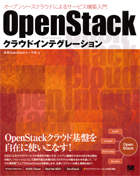
\includegraphics[height=15mm]{images/OpenStack_Integration_book.png}~
\includegraphics[height=15mm]{images/InfraCI_book.png}
      \begin{itemize}
      \item \href{https://www.amazon.co.jp/dp/4798139785/}{\scriptsize{OpenStack
        Cloud Integration (OpenStack クラウドインテグレーション)}}
      \item \href{https://www.amazon.co.jp/dp/4798155128/}{\scriptsize{Infra CI
        Pragmatic Guide - Ansible/GitLab (インフラ CI 実践ガイド)}} (as a reviewer)
      \end{itemize}
    \item Hobby: Bike(BMC SLR02), Clouds(OpenStack...), Diet(Low-carb), etc.
    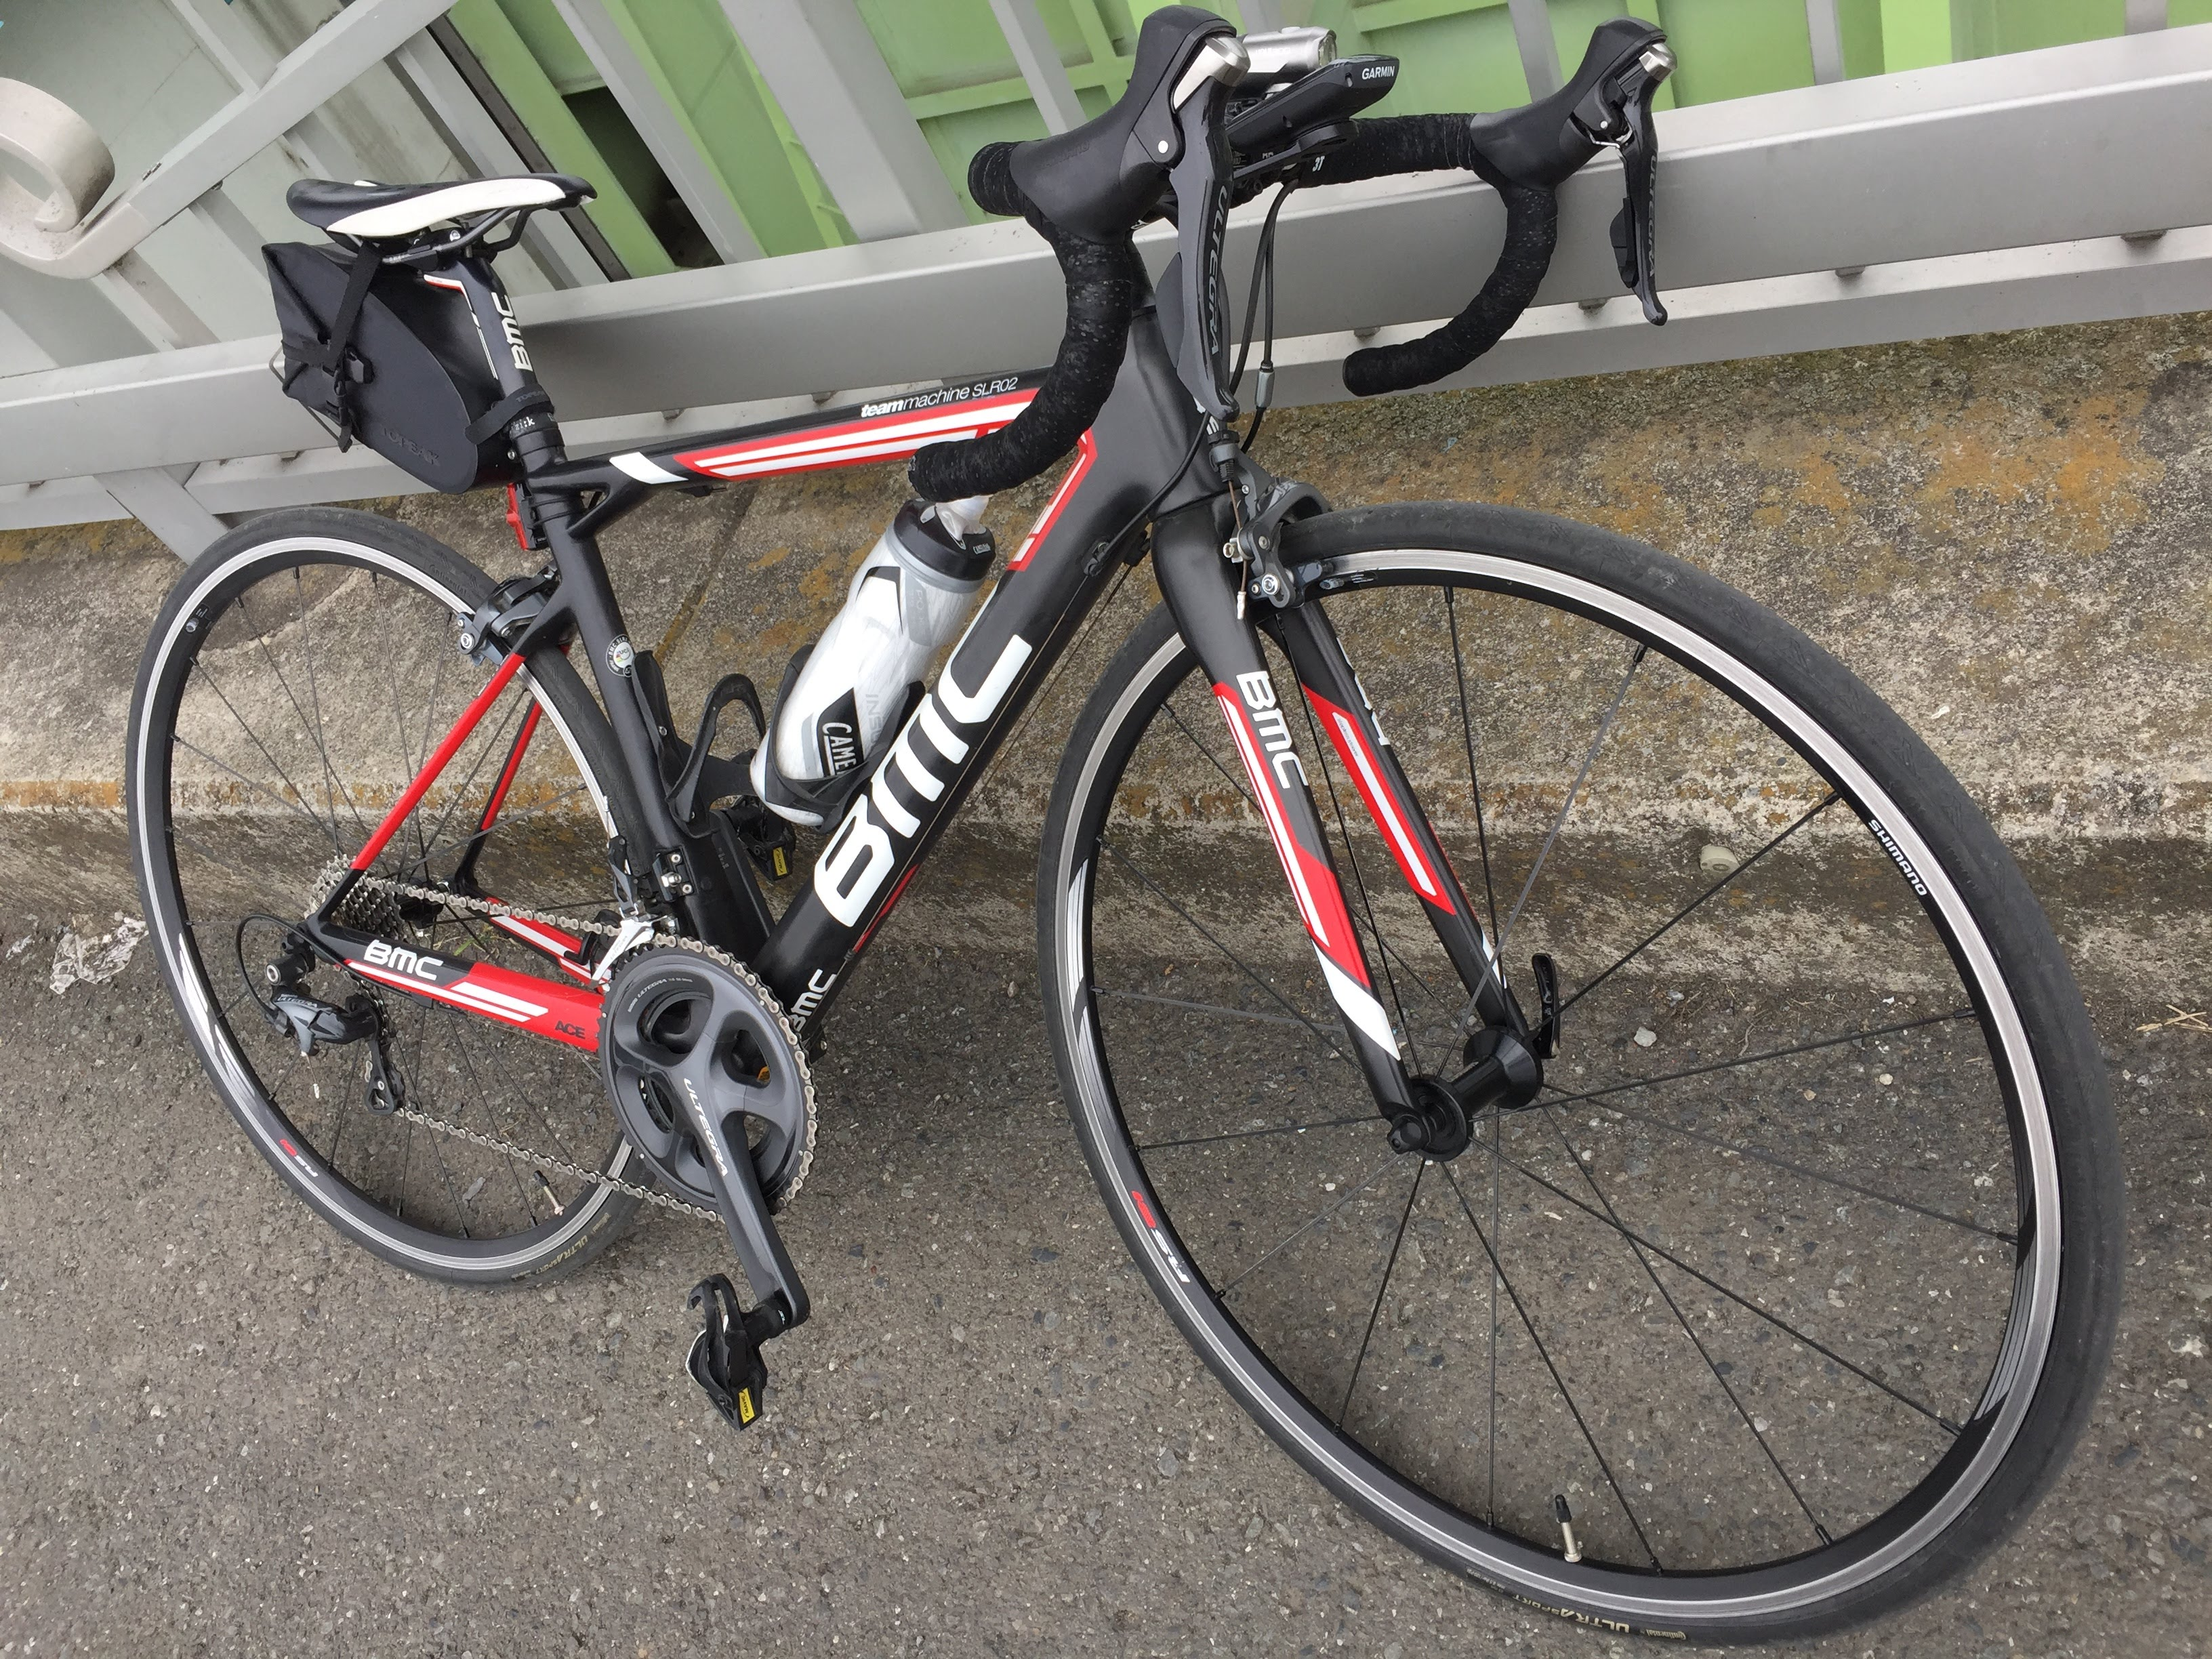
\includegraphics[height=20mm]{images/my-bike.jpg}~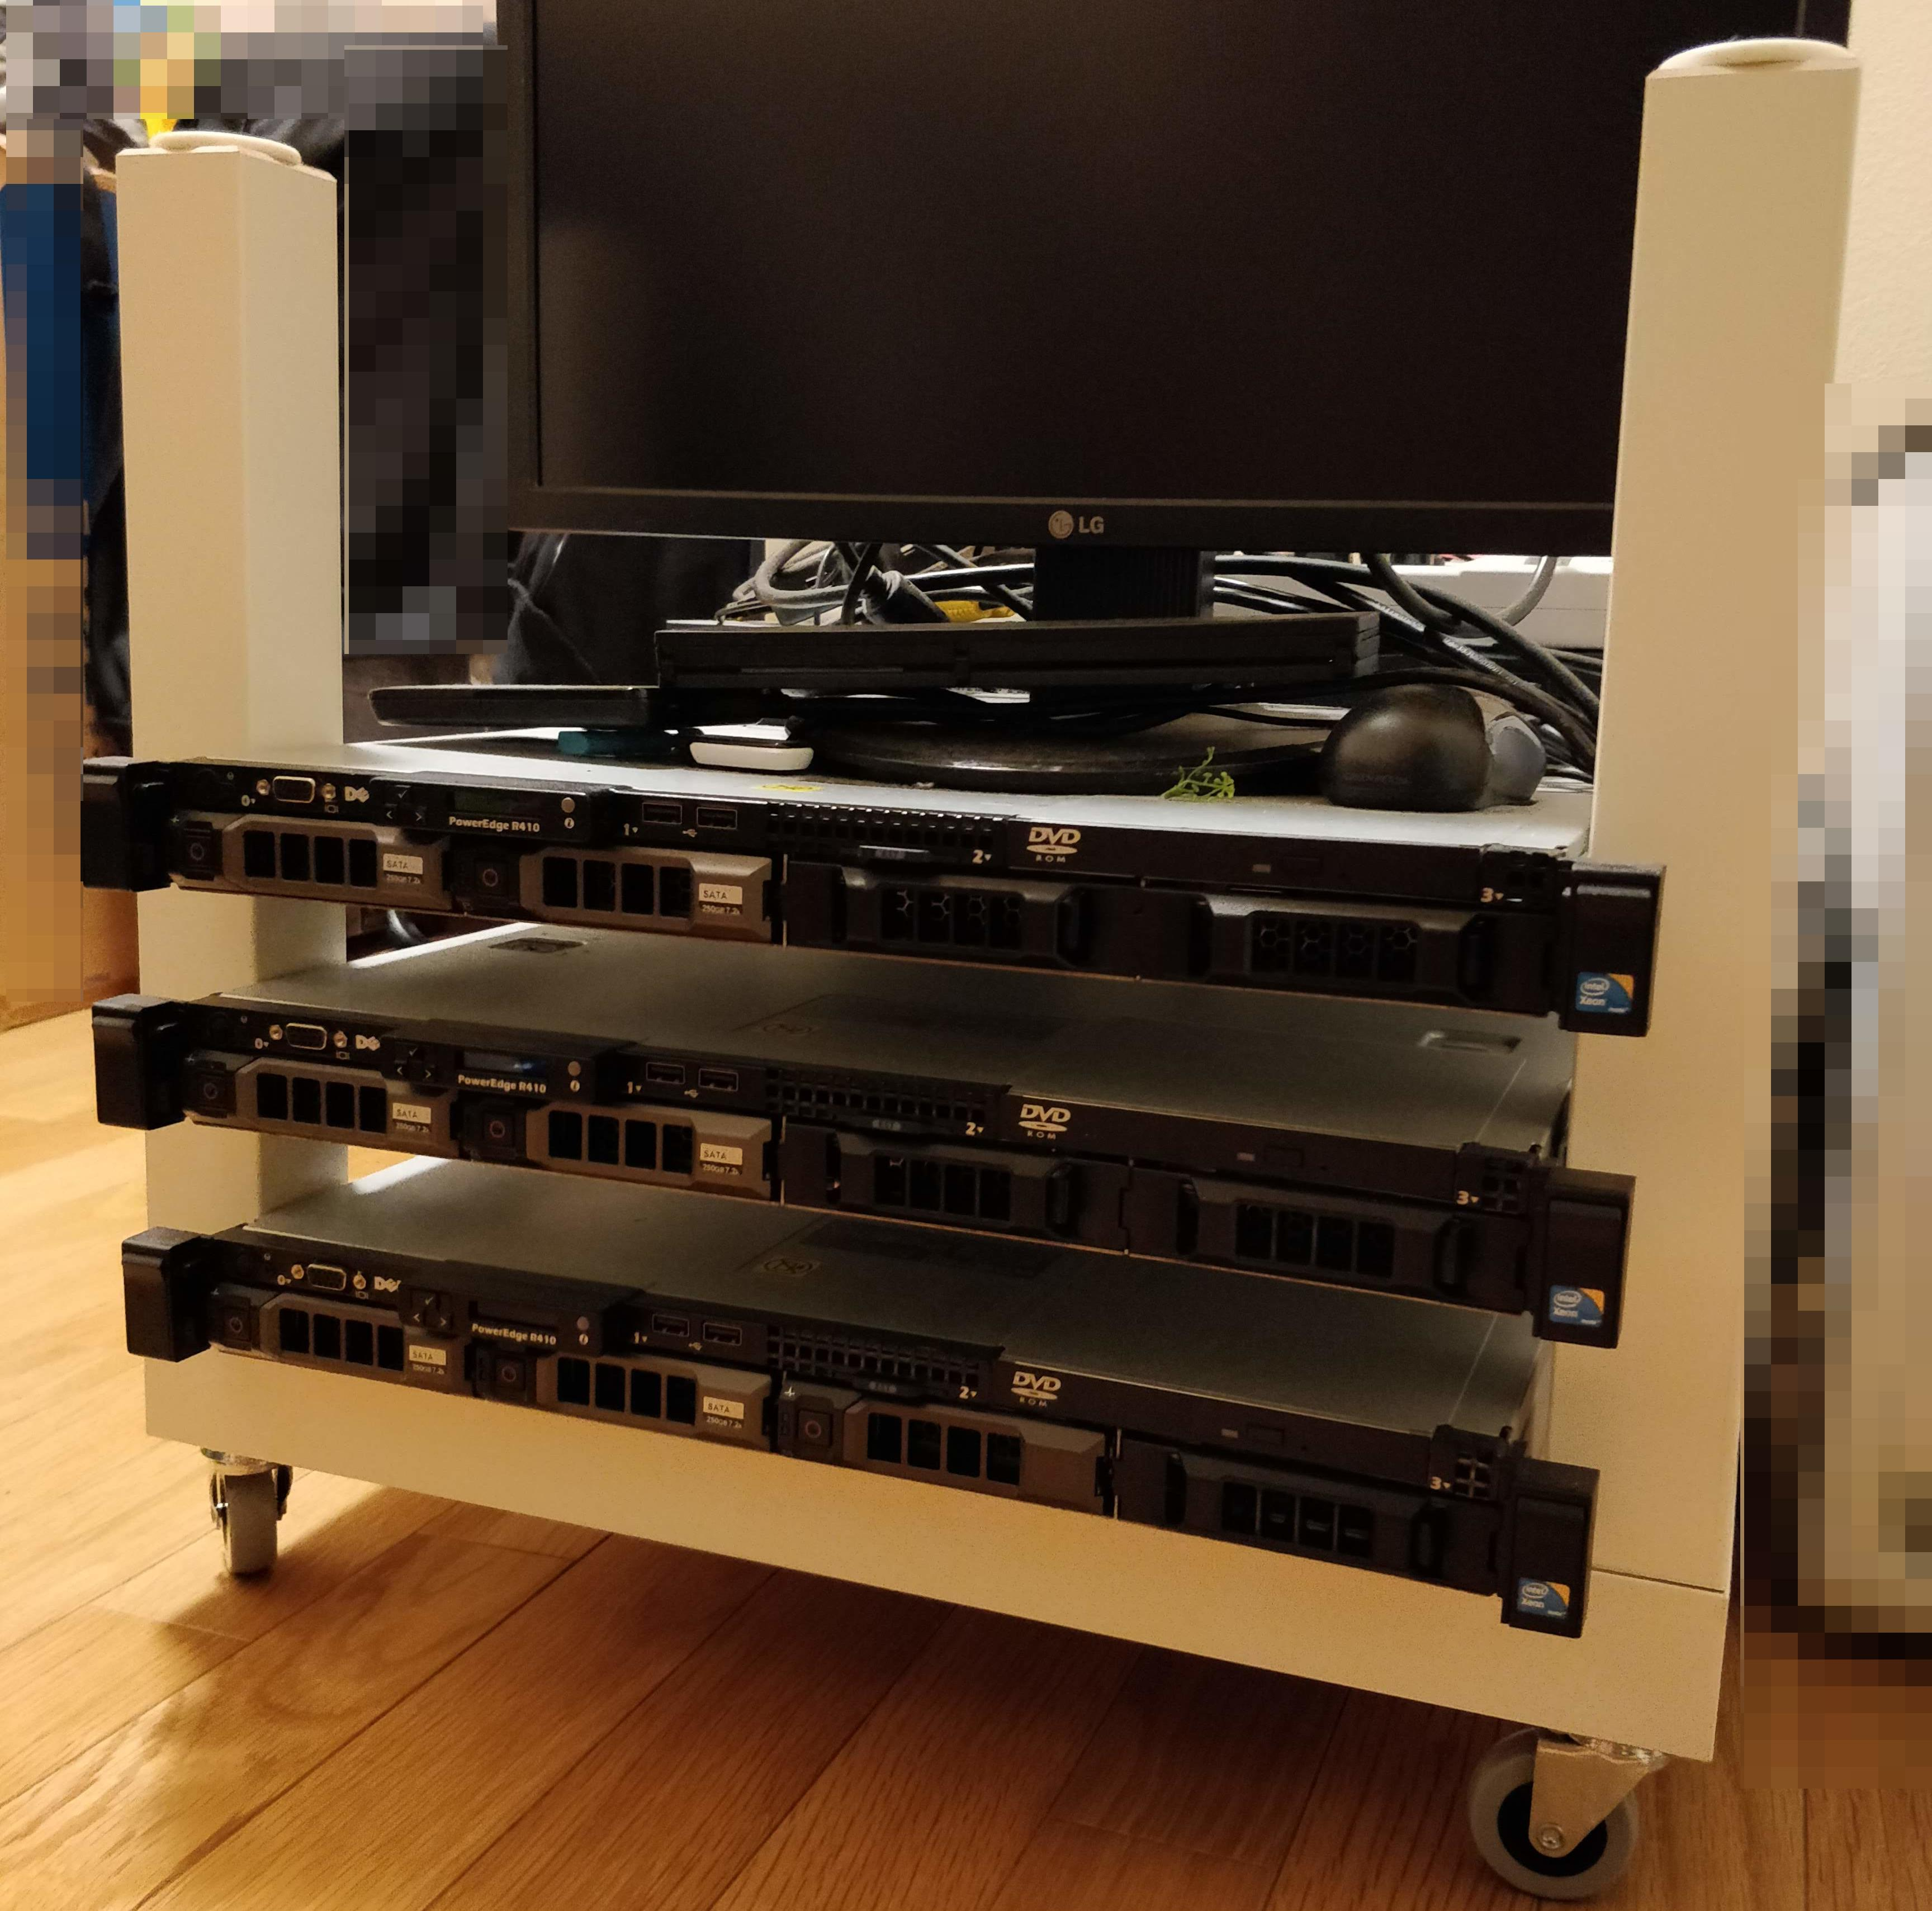
\includegraphics[height=20mm]{images/server_front.jpg}~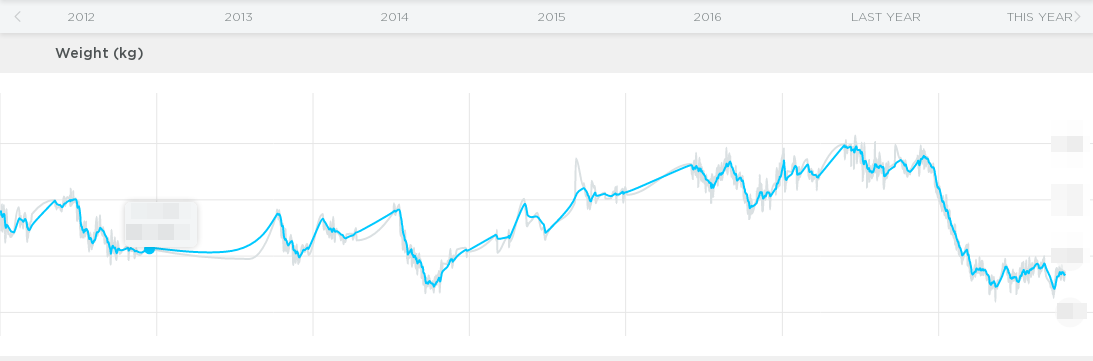
\includegraphics[height=20mm]{images/my-weight.png}
  \end{itemize}
\end{frame}

\section{Goal of today}
\begin{frame}
  \frametitle{今日のゴール}
  \begin{itemize}
    \item ``Kubernetes The Hard Way'' とは何かを理解する
    \item 自分で ``Kubernetes The Hard Way'' やってみたい!(と思ってもらう)
  \end{itemize}
\end{frame}

\section{Introduction}
\begin{frame}
  \frametitle{こんなこと感じませんか?}
  minikube, kubeadm, Rancher, GKE/AKS/EKS, etc. 使って k8s 使ってみたけど..
  \begin{itemize}
    \item どんなコンポーネントがあるのか知りたい
    \item 障害が起きたらデバッグできるようにしたい
    \item 自分好みの Kubernetes クラスタを構築したい
    \item 最近の Kubernetes は簡単すぎる
    \item もっと苦労したい!
  \end{itemize}
\end{frame}

\begin{frame}
  \frametitle{そんなあなたに}
  \begin{itemize}
    \item[] \Huge{``Kubernetes the Hard Way''}\large{}
    \item \url{https://github.com/kelseyhightower/kubernetes-the-hard-way}
    \item[] 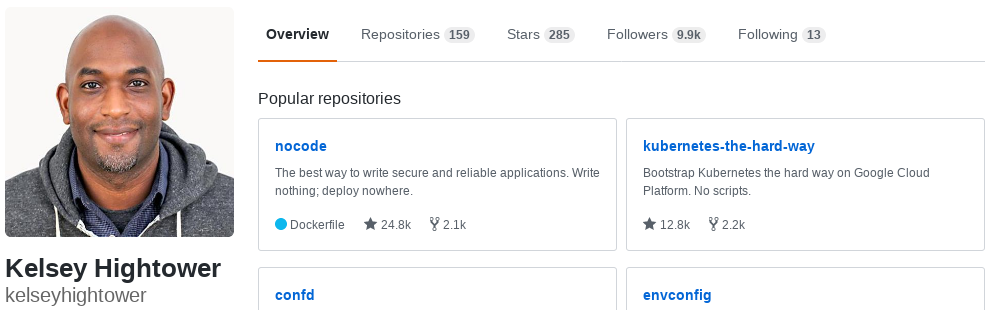
\includegraphics[height=40mm]{images/kelseyhightower_overview.png}
  \end{itemize}
\end{frame}

\section{What is k8s the hard way?}
\begin{frame}
  \frametitle{``Kubernetes the Hard Way'' ?}
  \begin{itemize}
    \item Kubernetes 学習用のチュートリアル資料
    \item Apache License Version 2.0
    \item 全14章で構成されるドキュメント
  \end{itemize}
\end{frame}

\begin{frame}
  \frametitle{``Kubernetes the Hard Way'' ? - クラスタ構成コンポーネント}
  \begin{itemize}
    \item \href{https://github.com/kubernetes/kubernetes}{Kubernetes} 1.12.0
    \item \href{https://github.com/containerd/containerd}{containerd Container Runtime} 1.2.0-rc.0
    \item \href{https://github.com/google/gvisor}{gVisor} 50c283b9f56bb7200938d9e207355f05f79f0d17
    \item \href{https://github.com/containernetworking/cni}{CNI Container Networking} 0.6.0
    \item \href{https://github.com/etcd-io/etcd}{etcd} v3.3.9
    \item \href{https://github.com/coredns/coredns}{CoreDNS} v1.2.2

  \end{itemize}
\end{frame}


\section{What is k8s the hard way?}
\begin{frame}
  \frametitle{``Kubernetes the Hard Way'' ? - 概略}
  \begin{enumerate}
    \item Prerequisites
    \item Installing the Client Tools
    \item Provisioning Compute Resources
    \item Provisioning a CA and Generating TLS Certificates
    \item Generating Kubernetes Configuration Files for Authentication
    \item Generating the Data Encryption Config and Key
    \item Bootstrapping the etcd Cluster
    \item Bootstrapping the Kubernetes Control Plane
    \item Bootstrapping the Kubernetes Worker Nodes
    \item Configuring kubectl for Remote Access
    \item Provisioning Pod Network Routes
    \item Deploying the DNS Cluster Add-on
    \item Smoke Test
    \item Cleaning Up
  \end{enumerate}
\end{frame}

\section{What is k8s the hard way?}
\begin{frame}
  \frametitle{``Kubernetes the Hard Way'' ? - 一部紹介}
  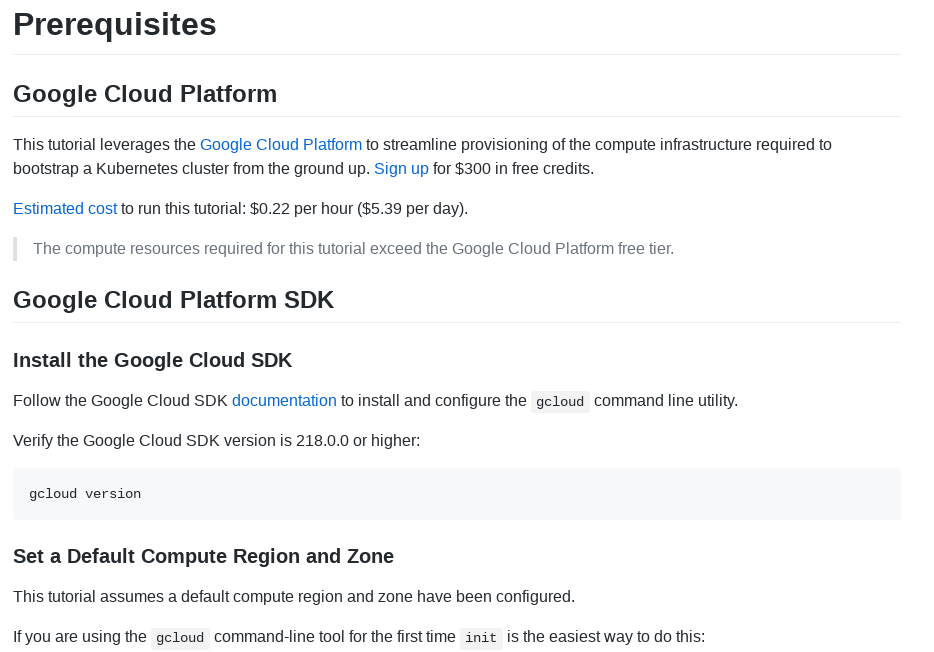
\includegraphics[height=75mm]{images/screenshot-k8s-the-hard-way.png}
\end{frame}

\begin{frame}
  \frametitle{前提条件}
  \begin{itemize}
    \item GCP上で動作することが想定されている
    \item n1-standard-1(vCPU*1,MEM: 3.75GB) * 6
    \item[] -> Controller * 3 + Worker * 3 + Load Balancer
  \end{itemize}
\end{frame}

\begin{frame}
  \frametitle{アーキテクチャ・コンポーネント - どんな k8s が出来上がる?}
  \centering{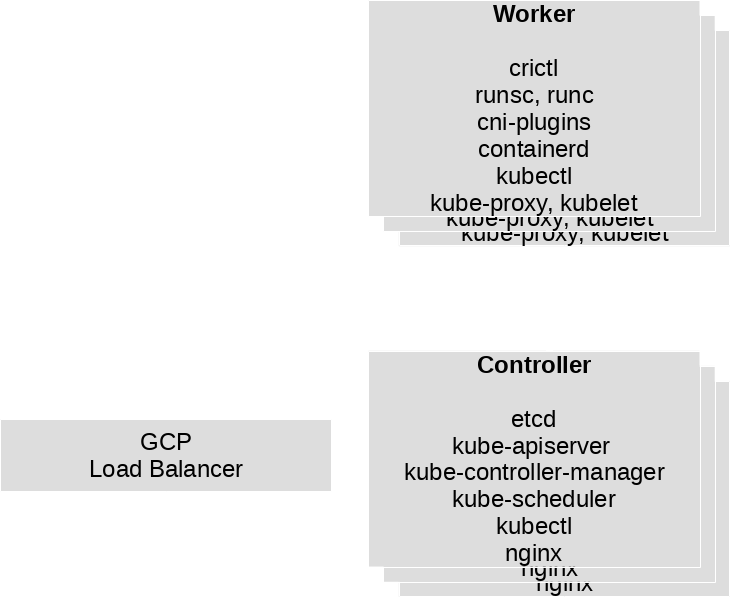
\includegraphics[height=75mm]{images/architecture.png}}
\end{frame}

\section{Conclusion}
\begin{frame}
  \frametitle{結果}
  \begin{itemize}
    \item 時間: 2.5H, コスト: 100円以下
    \item 「Hard Way」と書かれているものの、実行自体はすんなり
    \item[]  -> じっくりやっても 2.5H 以下
    \item とは言え、なぞってやっただけではやっぱり理解しきれない
    \item[] -> 自分が動かしたい環境で、試行錯誤・カスタマイズ、動かす必要あり
  \end{itemize}
\end{frame}

\section{Conclusion}
\begin{frame}
  \frametitle{困ったこと・気づき・小ネタ}
  \begin{itemize}
    \item 自分が動かしたい環境で、試行錯誤・カスタマイズで理解深める
    \item \href{https://github.com/masayukig/k8s-the-hard-way-script}{Bash script} 作りました
    \item[] -> \url{https://github.com/masayukig/k8s-the-hard-way-script}
    \item あくまで検証用 (例: Workerノードの追加・削除はちょっと面倒くさそう(?))
    \item 書籍・Web情報などとともに行き来しながら学習すると、良さそう
    \begin{itemize}
      \item
      \href{https://book.impress.co.jp/books/1118101055}{Kubernetes完全ガイド}
      \item
      \href{https://www.shoeisha.co.jp/book/detail/9784798155371}{コンテナ・ベース・オーケストレーション}
      \item
      \href{https://www.oreilly.co.jp/books/9784873118406/}{入門 Kubernetes}
      \item[]
      \item[] 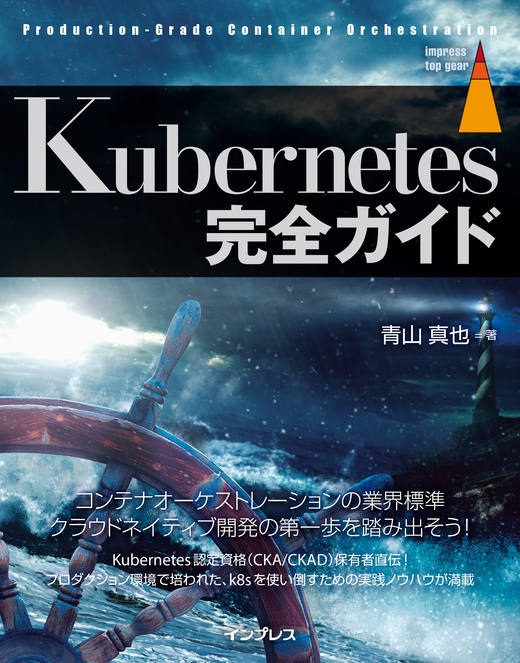
\includegraphics[height=20mm]{images/kubernetes_complete_guide.jpg}
       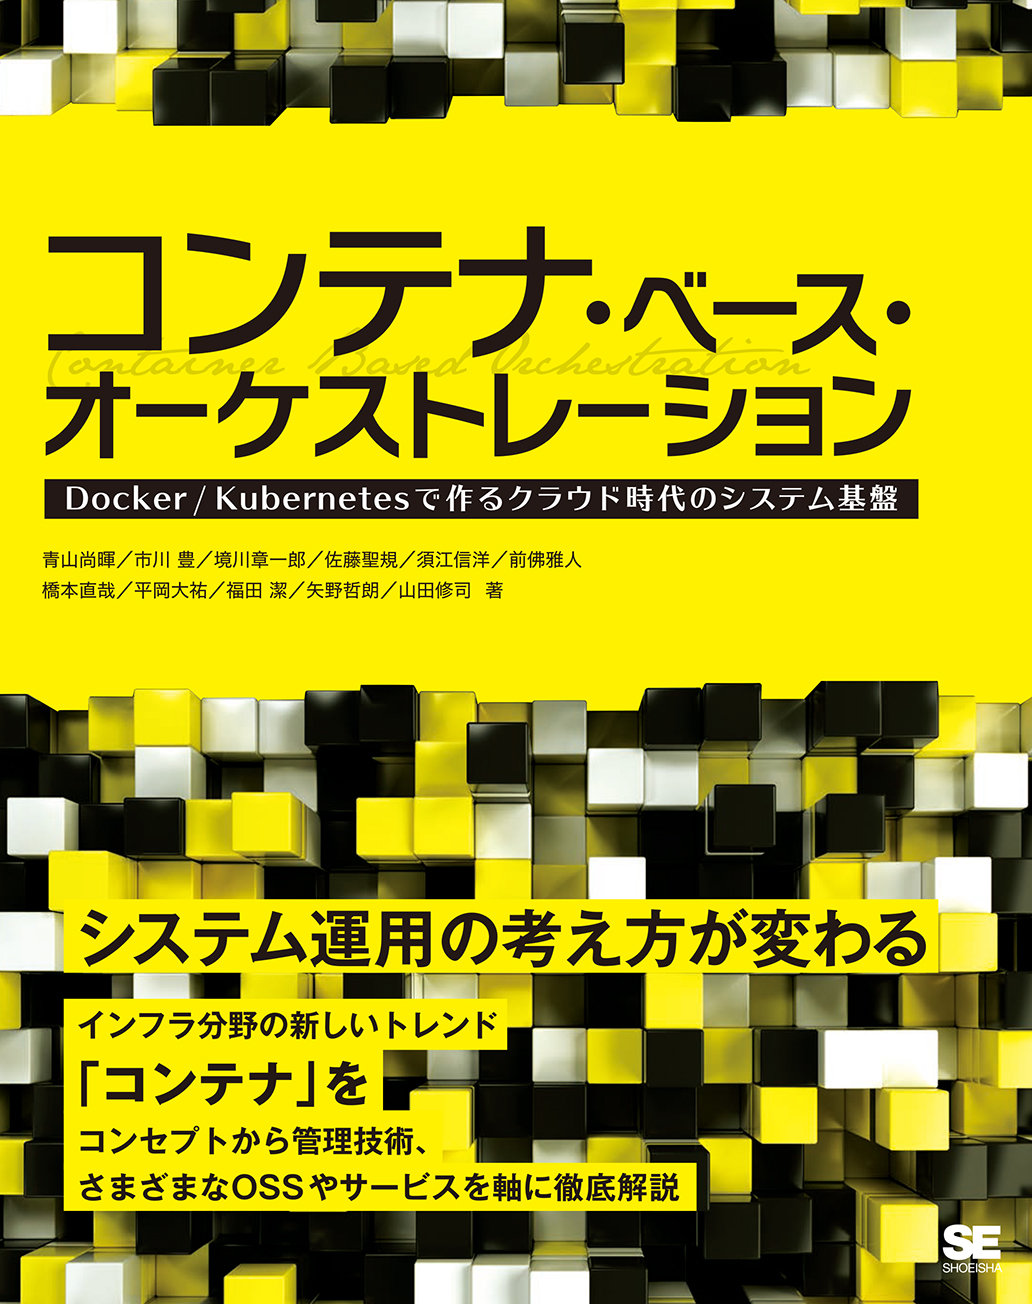
\includegraphics[height=20mm]{images/container_based_orchestration.jpg}
       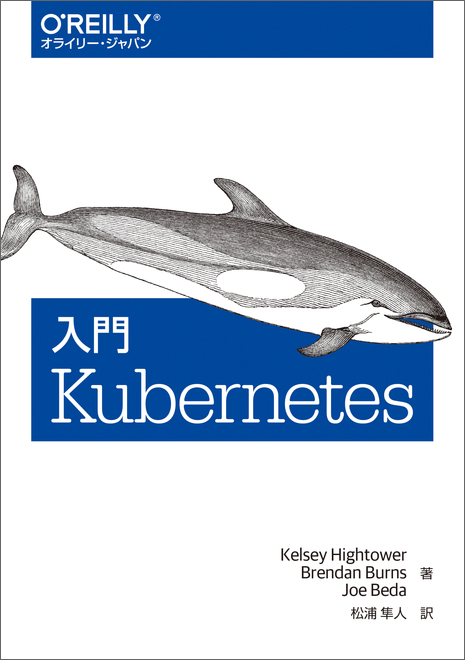
\includegraphics[height=20mm]{images/kubernetes_up_and_running.jpeg}
    \end{itemize}
  \end{itemize}
\end{frame}

\section{Future Plan}
\begin{frame}
  \frametitle{今後の(私の)展望}
  \begin{itemize}
    \item Baremetal, libvirt/KVM, Vagrant, OpenStack 上で動かす!
    \item[] どこのご家庭にもありますよね?
  \end{itemize}
\end{frame}

\section{Appendix}
\begin{frame}
  \frametitle{まとめ}
  \begin{itemize}
    \item 「Hard Way」だけど、実行自体はすんなり: じっくりやっても2.5H
    \item とは言え、コピペでやっただけでは理解しきれない
    \item[] -> 自分が動かしたい環境で、試行錯誤・カスタマイズ・動かす必要
    \item[] 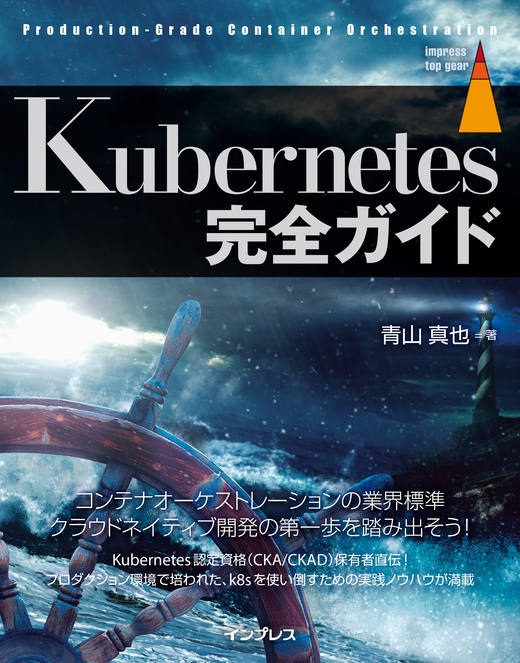
\includegraphics[height=20mm]{images/kubernetes_complete_guide.jpg}
       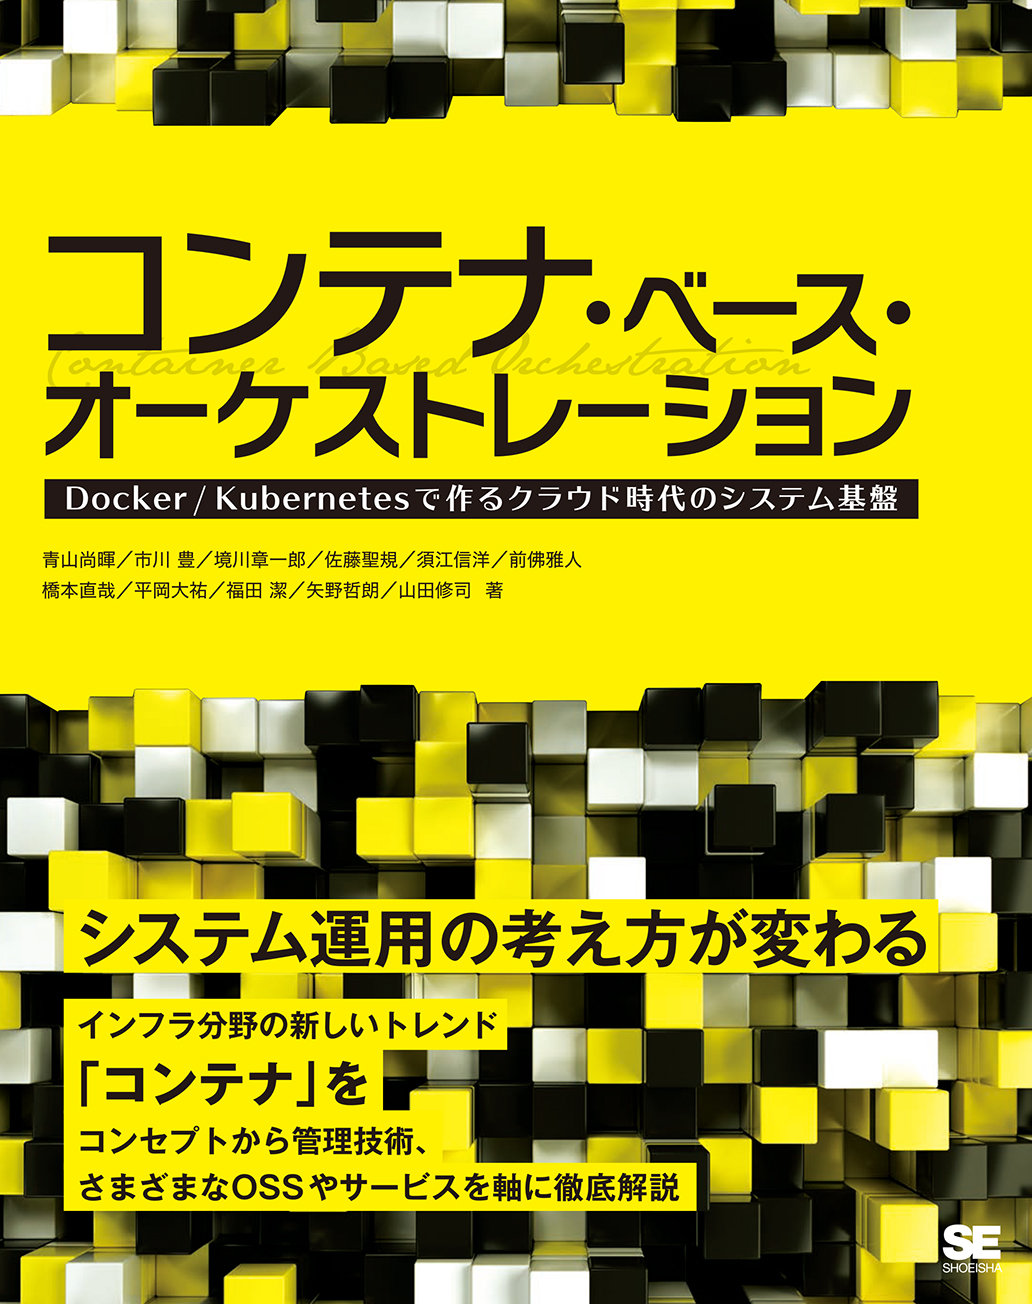
\includegraphics[height=20mm]{images/container_based_orchestration.jpg}
       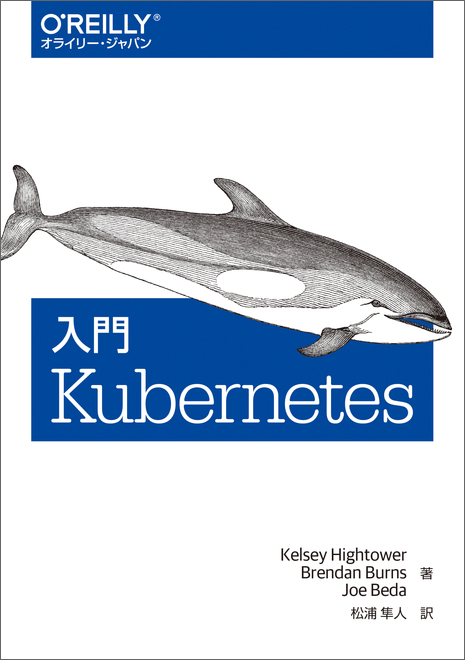
\includegraphics[height=20mm]{images/kubernetes_up_and_running.jpeg}
    \item Open Source のメリットを最大限に活かしましょう!
  \end{itemize}
  Appendix
  \begin{itemize}
      \item Slides: \url{https://bit.ly/k8s-the-hard-way-jkd-v1812}
      \item Contact info: \texttt{masayukig on
        \href{https://freenode.net/}{Freenode},
        \href{https://github.com/masayukig}{GitHub},
        \href{https://twitter.com/masayukig}{Twitter},
        \href{https://www.linkedin.com/in/masayukig/}{LinkedIn}}
      \item Kubernetes The Hard Way: \url{https://github.com/kelseyhightower/kubernetes-the-hard-way}
  \end{itemize}
\end{frame}

\end{document}
